\section{予測符号化}
\subsection{観測世界の階層的予測}
\textbf{階層的予測符号化(hierarchical predictive coding; HPC)}\index{かいそうてきよそくふごうか(hierarchical predictive coding; HPC)@階層的予測符号化(hierarchical predictive coding; HPC)} は\cite{Rao1999-zv}により導入された.構築するネットワークは入力層を含め,3層のネットワークとする.LGNへの入力として画像 $\mathbf{x} \in \mathbb{R}^{n_0}$を考える.画像 $\mathbf{x}$ の観測世界における隠れ変数,すなわち\textbf{潜在変数}\index{せんざいへんすう@潜在変数} (latent variable)を$\mathbf{r} \in \mathbb{R}^{n_1}$とし,ニューロン群によって発火率で表現されているとする (真の変数と $\mathbf{r}$は異なるので文字を分けるべきだが簡単のためにこう表す).このとき,


\begin{equation}
\mathbf{x} = f(\mathbf{U}\mathbf{r}) + \boldsymbol{\epsilon}
\end{equation}


が成立しているとする.ただし,$f(\cdot)$は活性化関数 (activation function),$\mathbf{U} \in \mathbb{R}^{n_0 \times n_1}$は重み行列である.
$\boldsymbol{\epsilon} \in \mathbb{R}^{n_0}$ は $\mathcal{N}(\mathbf{0}, \sigma^2 \mathbf{I})$ からサンプリングされるとする.

潜在変数 $\mathbf{r}$はさらに高次 (higher-level)の潜在変数 $\mathbf{r}^h$により,次式で表現される.


\begin{equation}
\mathbf{r} = \mathbf{r}^{td}+\boldsymbol{\epsilon}^{td}=f(\mathbf{U}^h \mathbf{r}^h)+\boldsymbol{\epsilon}^{td}
\end{equation}


ただし,Top-downの予測信号を $\mathbf{r}^{td}\triangleqf(\mathbf{U}^h \mathbf{r}^h)$とした.また,$\mathbf{r}^{td} \in \mathbb{R}^{n_1}$, $\mathbf{r}^{h} \in \mathbb{R}^{n_2}$, $\mathbf{U}^h \in \mathbb{R}^{n_1 \times n_2}$ である.
$\boldsymbol{\epsilon}^{td} \in \mathbb{R}^{n_1}$は$\mathcal{N}(\mathbf{0}$, $\sigma_{td}^2 \mathbf{I}$) からサンプリングされるとする.

話は飛ぶが,Predictive codingのネットワークの特徴は
\begin{itemize}
\item 階層的な構造
\item 高次による低次の予測 (Feedback or Top-down信号)
\item 低次から高次への誤差信号の伝搬 (Feedforward or Bottom-up 信号)
\end{itemize}

である.ここまでは高次表現による低次表現の予測,というFeedback信号について説明してきたが,この部分はSparse codingでも同じである.それではPredictive codingのもう一つの要となる,低次から高次への予測誤差の伝搬というFeedforward信号はどのように導かれるのだろうか.結論から言えば,これは\textbf{復元誤差 (reconstruction error)の最小化を行う再帰的ネットワーク (recurrent network)を考慮することで自然に導かれる}\index{ふくげんごさ (reconstruction error)のさいしょうかをおこなうさいきてきねっとわーく (recurrent network)をこうりょすることでしぜんにみちびかれる@復元誤差 (reconstruction error)の最小化を行う再帰的ネットワーク (recurrent network)を考慮することで自然に導かれる}.
\subsection{損失関数と学習則}
\subsubsection{事前分布の設定}
$\mathbf{r}$の事前分布$p(\mathbf{r})$はCauchy分布を用いる.$p(\mathbf{r})$の負の対数事前分布を$g(\mathbf{r})\triangleq-\log p(\mathbf{r})$としておく.


\begin{align}
p(\mathbf{r})&=\prod_i p(r_i)=\prod_i \exp\left[-\alpha \ln(1+r_i^2)\right]\\
g(\mathbf{r})&=-\ln p(\mathbf{r})=\alpha \sum_i \ln(1+r_i^2)\\
g'(\mathbf{r})&=\frac{\partial g(\mathbf{r})}{\partial \mathbf{r}}=\left[\frac{2\alpha r_i}{1+r_i^2}\right]_i
\end{align}


次に重み行列$\mathbf{U}$の事前分布 $p(\mathbf{U})$はGaussian分布とする.$p(\mathbf{U})$の負の対数事前分布を$h(\mathbf{U})\triangleq-\ln p(\mathbf{U})$とすると,次のように表される.


\begin{align}
p(\mathbf{U})&=\exp(-\lambda\|\mathbf{U}\|^2_F)\\
h(\mathbf{U})&=-\ln p(\mathbf{U})=\lambda\|\mathbf{U}\|^2_F\\
h'(\mathbf{U})&=\frac{\partial h(\mathbf{U})}{\partial \mathbf{U}}=2\lambda \mathbf{U}
\end{align}


ただし,$\|\cdot \| _ F^2$はフロベニウスノルムを意味する.

\subsubsection{損失関数の設定}
Sparse codingと同様に考えることにより,損失関数 $E$を次のように定義する.


\begin{align}
E=\underbrace{\frac{1}{\sigma^{2}}\|\mathbf{x}-f(\mathbf{U} \mathbf{r})\|^2+\frac{1}{\sigma_{t d}^{2}}\left\|\mathbf{r}-f(\mathbf{U}^h \mathbf{r}^h)\right\|^2}_{\text{reconstruction error}}+\underbrace{g(\mathbf{r})+g(\mathbf{r}^{h})+h(\mathbf{U})+h(\mathbf{U}^h)}_{\text{sparsity penalty}}
\end{align}


潜在変数 $\mathbf{r}, \mathbf{r}^h$ と 重み行列 $\mathbf{U}, \mathbf{U}^h$ のそれぞれに事前分布を仮定しているため,これらについてのMAP推定を行うことに相当する.

\subsubsection{再帰ネットワークの更新則}
簡単のために$\mathbf{z}\triangleq\mathbf{U}\mathbf{r}, \mathbf{z}^h\triangleq\mathbf{U}^h\mathbf{r}^h$とする.


\begin{align}
\frac{d \mathbf{r}}{d t}&=-\frac{k_{1}}{2} \frac{\partial E}{\partial \mathbf{r}}=k_{1}\cdot\Bigg(\frac{1}{\sigma^{2}} \mathbf{U}^{T}\bigg[\frac{\partial f(\mathbf{z})}{\partial \mathbf{z}}\odot\underbrace{(\mathbf{x}-f(\mathbf{z}))}_{\text{bottom-up error}}\bigg]-\frac{1}{\sigma_{t d}^{2}}\underbrace{\left(\mathbf{r}-f(\mathbf{z}^h)\right)}_{\text{top-down error}}-\frac{1}{2}g'(\mathbf{r})\Bigg)\\
\frac{d \mathbf{r}^h}{d t}&=-\frac{k_{1}}{2} \frac{\partial E}{\partial \mathbf{r}^h}=k_{1}\cdot\Bigg(\frac{1}{\sigma_{t d}^{2}}(\mathbf{U}^h)^\top\bigg[\frac{\partial f(\mathbf{z}^h)}{\partial \mathbf{z}^h}\odot\underbrace{\left(\mathbf{r}-f(\mathbf{z}^h)\right)}_{\text{bottom-up error}}\bigg]-\frac{1}{2}g'(\mathbf{r}^h)\Bigg)
\end{align}


ただし,$k_1$は更新率 (updating rate)である.または,発火率の時定数を$\tau\triangleq1/k_1$として,$k_1$は発火率の時定数$\tau$の逆数であると捉えることもできる.ここで1番目の式において,中間表現 $\mathbf{r}$ のダイナミクスはbottom-up errorとtop-down errorで記述されている.このようにbottom-up errorが $\mathbf{r}$ への入力となることは自然に導出される.なお,top-down errorに関しては高次からの予測 (prediction)の項 $f(\mathbf{x}^h)$とleaky-integratorとしての項 $-\mathbf{r}$に分割することができる.また$\mathbf{U}^\top, (\mathbf{U}^h)^\top$は重み行列の転置となっており,bottom-upとtop-downの投射において対称な重み行列を用いることを意味している.$-g'(\mathbf{r})$は発火率を抑制してスパースにすることを目的とする項だが,無理やり解釈をすると自己再帰的な抑制と言える.
\subsubsection{画像データの読み込み}
「スパース符号化」と同様にデータは\url{http://www.rctn.org/bruno/sparsenet/}からダウンロードできるファイルを用いる.
\lstinputlisting[language=julia]{./text/energy-based-model/predictive-coding/003.jl}
\subsubsection{モデルの定義}
必要なパッケージを読み込む.
\lstinputlisting[language=julia]{./text/energy-based-model/predictive-coding/005.jl}
モデルを定義する.
\lstinputlisting[language=julia]{./text/energy-based-model/predictive-coding/007.jl}
パラメータを更新する関数を定義する.
\lstinputlisting[language=julia]{./text/energy-based-model/predictive-coding/009.jl}
入力に乗じるGaussianフィルタを定義する.
\lstinputlisting[language=julia]{./text/energy-based-model/predictive-coding/011.jl}
\lstinputlisting[language=julia]{./text/energy-based-model/predictive-coding/012.jl}
\begin{figure}[ht]
	\centering
	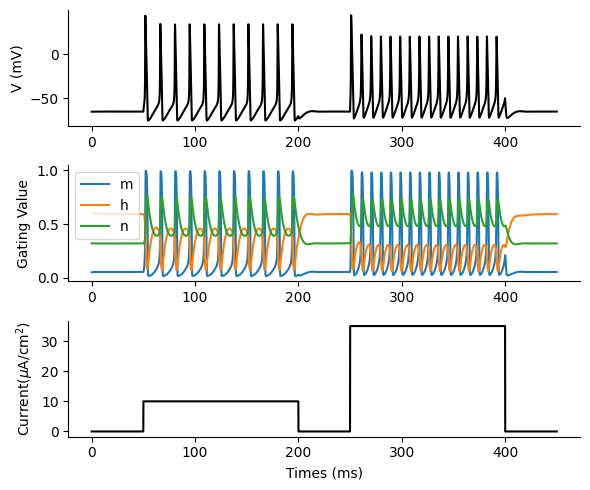
\includegraphics[scale=0.8, max width=\linewidth]{./fig/neuron-model/hodgkin-huxley/cell012.png}
	\caption{cell012.png}
	\label{cell012.png}
\end{figure}
損失関数を定義する.
\lstinputlisting[language=julia]{./text/energy-based-model/predictive-coding/014.jl}
シミュレーションを実行する関数を定義する.外側の\jl{for loop}では画像パッチの作成と\jl{r}の初期化を行う.内側の\jl{for loop}では\jl{r}が収束するまで更新を行い,収束したときに重み行列\jl{Phi}を更新する.
\lstinputlisting[language=julia]{./text/energy-based-model/predictive-coding/016.jl}
シミュレーションの実行をする
\lstinputlisting[language=julia]{./text/energy-based-model/predictive-coding/018.jl}
\subsubsection{訓練中の損失の描画}
訓練中の損失の変化を描画してみよう.損失が低下し,学習が進行したことが分かる.
\lstinputlisting[language=julia]{./text/energy-based-model/predictive-coding/020.jl}
\begin{figure}[ht]
	\centering
	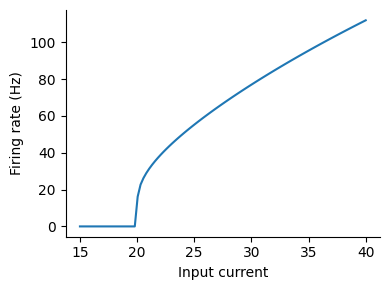
\includegraphics[scale=0.8, max width=\linewidth]{./fig/neuron-model/lif/cell020.png}
	\caption{cell020.png}
	\label{cell020.png}
\end{figure}
\subsubsection{重み行列 (受容野)の描画}
学習後の重み行列 ($\mathbf{U}$)を可視化してみよう.
\lstinputlisting[language=julia]{./text/energy-based-model/predictive-coding/022.jl}
\begin{figure}[ht]
	\centering
	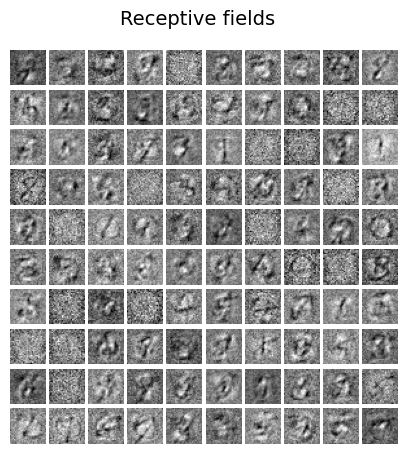
\includegraphics[scale=0.8, max width=\linewidth]{./fig/energy-based-model/boltzmann-machine/cell022.png}
	\caption{cell022.png}
	\label{cell022.png}
\end{figure}
白色が\textbf{ON領域}\index{ONりょういき@ON領域}(興奮),黒色が\textbf{OFF領域}\index{OFFりょういき@OFF領域}(抑制)を表す.Gaborフィルタ様の局所受容野が得られている.次に,Level2のニューロンの受容野は$\mathbf{U}$と$\mathbf{U}^h$の積を計算することで描画できる.
\lstinputlisting[language=julia]{./text/energy-based-model/predictive-coding/024.jl}
\begin{figure}[ht]
	\centering
	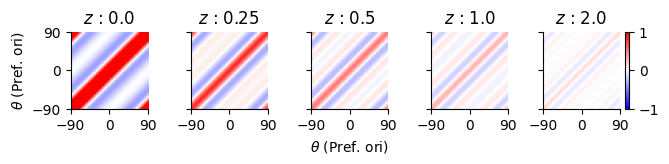
\includegraphics[scale=0.8, max width=\linewidth]{./fig/bayesian-brain/neural-sampling/cell024.png}
	\caption{cell024.png}
	\label{cell024.png}
\end{figure}
